%%%%%%%%%%%%%%%%%%%%%%%%%%%%%%%%%%%%%%%%%
% Programming/Coding Assignment
% LaTeX Template
%
% This template has been downloaded from:
% http://www.latextemplates.com
%
% Original author:
% Ted Pavlic (http://www.tedpavlic.com)
%
% Note:
% The \lipsum[#] commands throughout this template generate dummy text
% to fill the template out. These commands should all be removed when 
% writing assignment content.
%
% This template uses a Perl script as an example snippet of code, most other
% languages are also usable. Configure them in the "CODE INCLUSION 
% CONFIGURATION" section.
%
%%%%%%%%%%%%%%%%%%%%%%%%%%%%%%%%%%%%%%%%%

%----------------------------------------------------------------------------------------
%	PACKAGES AND OTHER DOCUMENT CONFIGURATIONS
%----------------------------------------------------------------------------------------

\documentclass{article}

\usepackage{fancyhdr} % Required for custom headers
\usepackage{lastpage} % Required to determine the last page for the footer
\usepackage{extramarks} % Required for headers and footers
\usepackage[usenames,dvipsnames]{color} % Required for custom colors
\usepackage{graphicx} % Required to insert images
\usepackage{listings} % Required for insertion of code
\usepackage{courier} % Required for the courier font
\usepackage{lipsum} % Used for inserting dummy 'Lorem ipsum' text into the template

% Margins
\topmargin=-0.45in
\evensidemargin=0in
\oddsidemargin=0in
\textwidth=6.5in
\textheight=9.0in
\headsep=0.25in

\linespread{1.1} % Line spacing

% Set up the header and footer
\pagestyle{fancy}
\lhead{\hmwkAuthorName} % Top left header
\chead{\hmwkClass\ (\hmwkClassInstructor\ \hmwkClassTime): \hmwkTitle} % Top center head
\rhead{\firstxmark} % Top right header
\lfoot{\lastxmark} % Bottom left footer
\cfoot{} % Bottom center footer
\rfoot{Page\ \thepage\ of\ \protect\pageref{LastPage}} % Bottom right footer
\renewcommand\headrulewidth{0.4pt} % Size of the header rule
\renewcommand\footrulewidth{0.4pt} % Size of the footer rule

\setlength\parindent{0pt} % Removes all indentation from paragraphs

%----------------------------------------------------------------------------------------
%	CODE INCLUSION CONFIGURATION
%----------------------------------------------------------------------------------------

\definecolor{MyDarkGreen}{rgb}{0.0,0.4,0.0} % This is the color used for comments
\lstloadlanguages{Perl} % Load Perl syntax for listings, for a list of other languages supported see: ftp://ftp.tex.ac.uk/tex-archive/macros/latex/contrib/listings/listings.pdf
\lstset{language=Perl, % Use Perl in this example
        frame=single, % Single frame around code
        basicstyle=\tiny\ttfamily, % Use small true type font
        keywordstyle=[1]\color{Blue}\bf, % Perl functions bold and blue
        keywordstyle=[2]\color{Purple}, % Perl function arguments purple
        keywordstyle=[3]\color{Blue}\underbar, % Custom functions underlined and blue
        identifierstyle=, % Nothing special about identifiers                                         
        commentstyle=\usefont{T1}{pcr}{m}{sl}\color{MyDarkGreen}\tiny, % Comments small dark green courier font
        stringstyle=\color{Purple}, % Strings are purple
        showstringspaces=false, % Don't put marks in string spaces
        tabsize=5, % 5 spaces per tab
        %
        % Put standard Perl functions not included in the default language here
        morekeywords={rand},
        %
        % Put Perl function parameters here
        morekeywords=[2]{on, off, interp},
        %
        % Put user defined functions here
        morekeywords=[3]{test},
       	%
        morecomment=[l][\color{Blue}]{...}, % Line continuation (...) like blue comment
        numbers=left, % Line numbers on left
        firstnumber=1, % Line numbers start with line 1
        numberstyle=\tiny\color{Blue}, % Line numbers are blue and small
        stepnumber=5 % Line numbers go in steps of 5
}

% Creates a new command to include a perl script, the first parameter is the filename of the script (without .pl), the second parameter is the caption
\newcommand{\pythonscript}[2]{
\begin{itemize}
\item[]\lstinputlisting[caption=#2,label=#1]{#1.py}
\end{itemize}
}

%----------------------------------------------------------------------------------------
%	DOCUMENT STRUCTURE COMMANDS
%	Skip this unless you know what you're doing
%----------------------------------------------------------------------------------------

% Header and footer for when a page split occurs within a problem environment
\newcommand{\enterProblemHeader}[1]{
\nobreak\extramarks{#1}{#1 continued on next page\ldots}\nobreak
\nobreak\extramarks{#1 (continued)}{#1 continued on next page\ldots}\nobreak
}

% Header and footer for when a page split occurs between problem environments
\newcommand{\exitProblemHeader}[1]{
\nobreak\extramarks{#1 (continued)}{#1 continued on next page\ldots}\nobreak
\nobreak\extramarks{#1}{}\nobreak
}

\setcounter{secnumdepth}{0} % Removes default section numbers
\newcounter{homeworkProblemCounter} % Creates a counter to keep track of the number of problems

\newcommand{\homeworkProblemName}{}
\newenvironment{homeworkProblem}[1][Problem \arabic{homeworkProblemCounter}]{ % Makes a new environment called homeworkProblem which takes 1 argument (custom name) but the default is "Problem #"
\stepcounter{homeworkProblemCounter} % Increase counter for number of problems
\renewcommand{\homeworkProblemName}{#1} % Assign \homeworkProblemName the name of the problem
\section{\homeworkProblemName} % Make a section in the document with the custom problem count
\enterProblemHeader{\homeworkProblemName} % Header and footer within the environment
}{
\exitProblemHeader{\homeworkProblemName} % Header and footer after the environment
}

\newcommand{\problemAnswer}[1]{ % Defines the problem answer command with the content as the only argument
\noindent\framebox[\columnwidth][c]{\begin{minipage}{0.98\columnwidth}#1\end{minipage}} % Makes the box around the problem answer and puts the content inside
}

\newcommand{\homeworkSectionName}{}
\newenvironment{homeworkSection}[1]{ % New environment for sections within homework problems, takes 1 argument - the name of the section
\renewcommand{\homeworkSectionName}{#1} % Assign \homeworkSectionName to the name of the section from the environment argument
\subsection{\homeworkSectionName} % Make a subsection with the custom name of the subsection
\enterProblemHeader{\homeworkProblemName\ [\homeworkSectionName]} % Header and footer within the environment
}{
\enterProblemHeader{\homeworkProblemName} % Header and footer after the environment
}

%----------------------------------------------------------------------------------------
%	NAME AND CLASS SECTION
%----------------------------------------------------------------------------------------

\newcommand{\hmwkTitle}{Assignment\ \#5} % Assignment title
\newcommand{\hmwkDueDate}{Thursday,\ October\ 16,\ 2014} % Due date
\newcommand{\hmwkClass}{CS\ 595} % Course/class
\newcommand{\hmwkClassTime}{4:20PM} % Class/lecture time
\newcommand{\hmwkClassInstructor}{Dr Nelson} % Teacher/lecturer
\newcommand{\hmwkAuthorName}{Victor Nwala} % Your name

%----------------------------------------------------------------------------------------
%	TITLE PAGE
%----------------------------------------------------------------------------------------

\title{
\vspace{2in}
\textmd{\textbf{\hmwkClass:\ \hmwkTitle}}\\
\normalsize\vspace{0.1in}\small{Due\ on\ \hmwkDueDate}\\
\vspace{0.1in}\large{\textit{\hmwkClassInstructor\ \hmwkClassTime}}
\vspace{3in}
}

\author{\textbf{\hmwkAuthorName}}
\date{} % Insert date here if you want it to appear below your name

%----------------------------------------------------------------------------------------

\begin{document}

\maketitle

%----------------------------------------------------------------------------------------
%	TABLE OF CONTENTS
%----------------------------------------------------------------------------------------

%\setcounter{tocdepth}{1} % Uncomment this line if you don't want subsections listed in the ToC

\newpage
\tableofcontents
\newpage

%----------------------------------------------------------------------------------------
%	PROBLEM 1
%----------------------------------------------------------------------------------------

% To have just one problem per page, simply put a \clearpage after each problem

\begin{homeworkProblem}
1.  Explore the friendship paradox for your Twitter account.  Since
Twitter has directional links (i.e., ``followers" and ``following"),
we'll be investigating if the people you follow (Twitter calls these
people ``friends") follow more people than you.  If you are following less than
50 people, use my twitter account ``phonedude\_mln" instead of your own.


\pythonscript{friendsList}{Python script to extract friends of ``phonedude\_mln" from twitter}
The script downloads the friends count of the friends of ``phonedude\_mln" and store the results in a file.


\problemAnswer{
\begin{center}
{ Figure 1: friendsList.py at work}
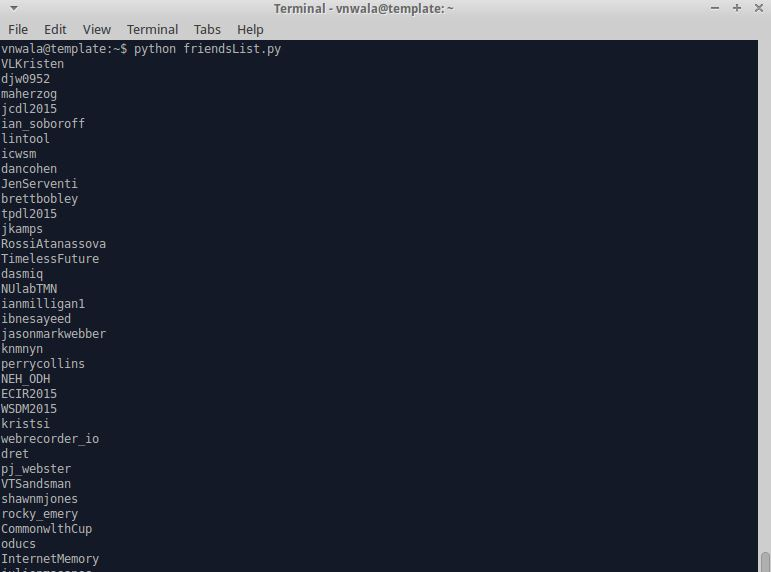
\includegraphics[width=0.75\columnwidth]{friendsList}
\end{center}
}








\problemAnswer{
\begin{center}
{ Figure 2: Twitter Friends Graph}
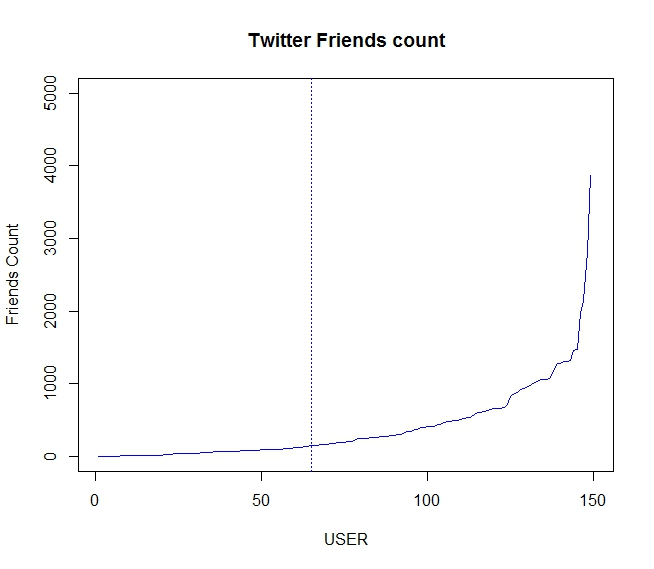
\includegraphics[width=0.75\columnwidth]{twitterFriends}



 
{Graph showing the friend count of ``phonedude\_mln" with vertical line showing his position, 65 on the user axis and a corresponding count of 148 friends}
\end{center}
}

\begin{table}[ht]
\caption{Twitter Friends Count Statistics}% title of Table
\centering% used for centering table
\begin{tabular}{c c c }% centered columns (3 columns)
\hline\hline %inserts double horizontal lines
MEAN & MEDIAN & STANDARD DEVITION\\[0.5ex]% inserts table
%heading
\hline% inserts single horizontal line

404.7919 & 191 & 545.7179 \\[1ex]% [1ex] adds vertical space
\hline%inserts single line
\end{tabular}
\label{table:nonlin}% is used to refer this table in the text
\end{table}

\end{homeworkProblem}

%----------------------------------------------------------------------------------------
%	PROBLEM 2
%----------------------------------------------------------------------------------------

\begin{homeworkProblem}
2.  Using your facebook account, repeat question \#1 (if you have greater than
50 friends).


To answer the question, I used the code credited to ``Alexander Nwala" to extract my friends from facebook and their respective friends count. 

\pythonscript{seleniumScrapePB}{Python script to extract friends of ``Victor Nwala" from Facebook}

\problemAnswer{
\begin{center}
{ Figure 3: seleniumScrapePB.py at work}
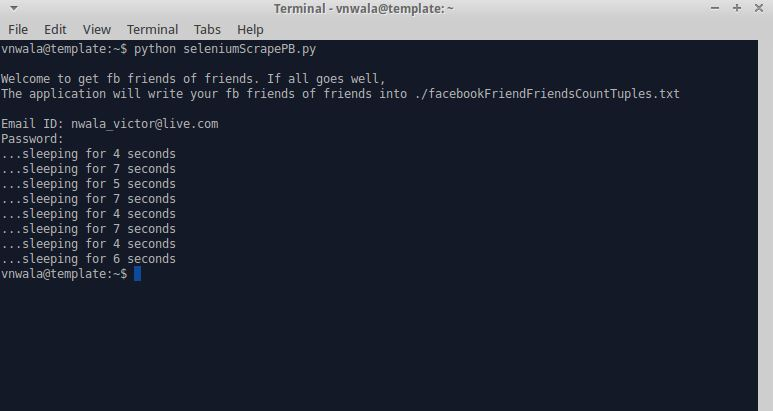
\includegraphics[width=0.75\columnwidth]{seleniumScrapePB}
\end{center}
}


\problemAnswer{
\begin{center}
{ Figure 4: Facebook Friends Graph}
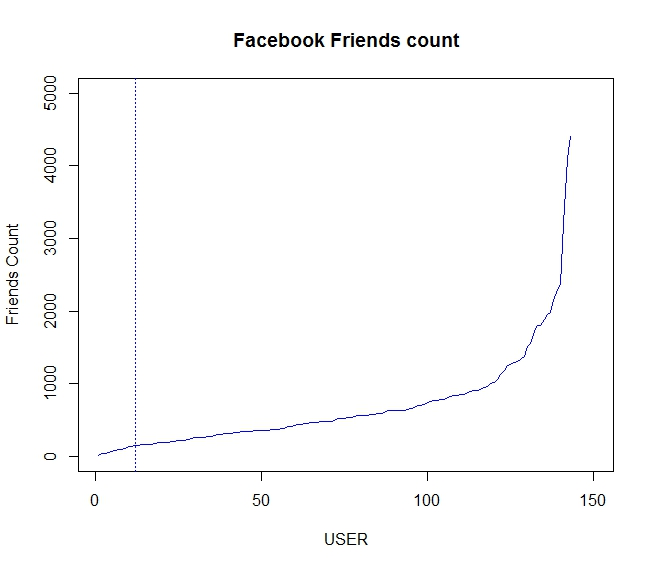
\includegraphics[width=0.75\columnwidth]{RplotFacebook}



 
{Graph showing the friend count of ``Victor Nwala" with vertical line showing his position, 12 on the user axis and a corresponding count of 155 friends}
\end{center}
}

\begin{table}[ht]
\caption{Facebook Friends Count Statistics}% title of Table
\centering% used for centering table
\begin{tabular}{c c c }% centered columns (3 columns)
\hline\hline %inserts double horizontal lines
MEAN & MEDIAN & STANDARD DEVITION\\[0.5ex]% inserts table
%heading
\hline% inserts single horizontal line

691.2238 & 490 & 681.5631 \\[1ex]% [1ex] adds vertical space
\hline%inserts single line
\end{tabular}
\label{table:nonlin}% is used to refer this table in the text
\end{table}


\end{homeworkProblem}

\clearpage

%----------------------------------------------------------------------------------------
%	OBSERVATIONS AND CONCLUSIONS
%----------------------------------------------------------------------------------------

In conclusion, the font size in my code listing is smaller than usual so that my code will all fit into the defined text area.
Secondly, the facebook extraction code, seleniumScrapePB.py extracts only friend counts of friends whose counts are visible.
Finally, the mean, median and standard deviation calculations where all done in Rstudio with a tool called, favstats. I also used the ``abline()" function to specify the exact locations for my vertical line on both graphs in Rstudio. I should also state that the ``Tweepy Documentation" was very helpful for problem 1. 


%----------------------------------------------------------------------------------------

\end{document}
